\documentclass[12pt, oneside]{extbook} % the document type needs to be change
\usepackage{geometry}
\usepackage{listings}
\usepackage{graphicx}
\usepackage[utf8]{inputenc}
\usepackage[T1]{fontenc}
\usepackage[italian]{babel}

\geometry{
    top = 1.5cm,
    bottom = 1.5cm,
    left = 2cm,
    right=2cm,
}

\begin{document}

\chapter*{VXLAN ed EVPN}

\section{Datacenter networks}
Le reti dei datacenter sono leggermente differenti rispetto a quelle degli ISP.
\\Le reti dei datacenter hanno una topologia di questo tipo:\\
\begin{figure}[h!]
    \centering
    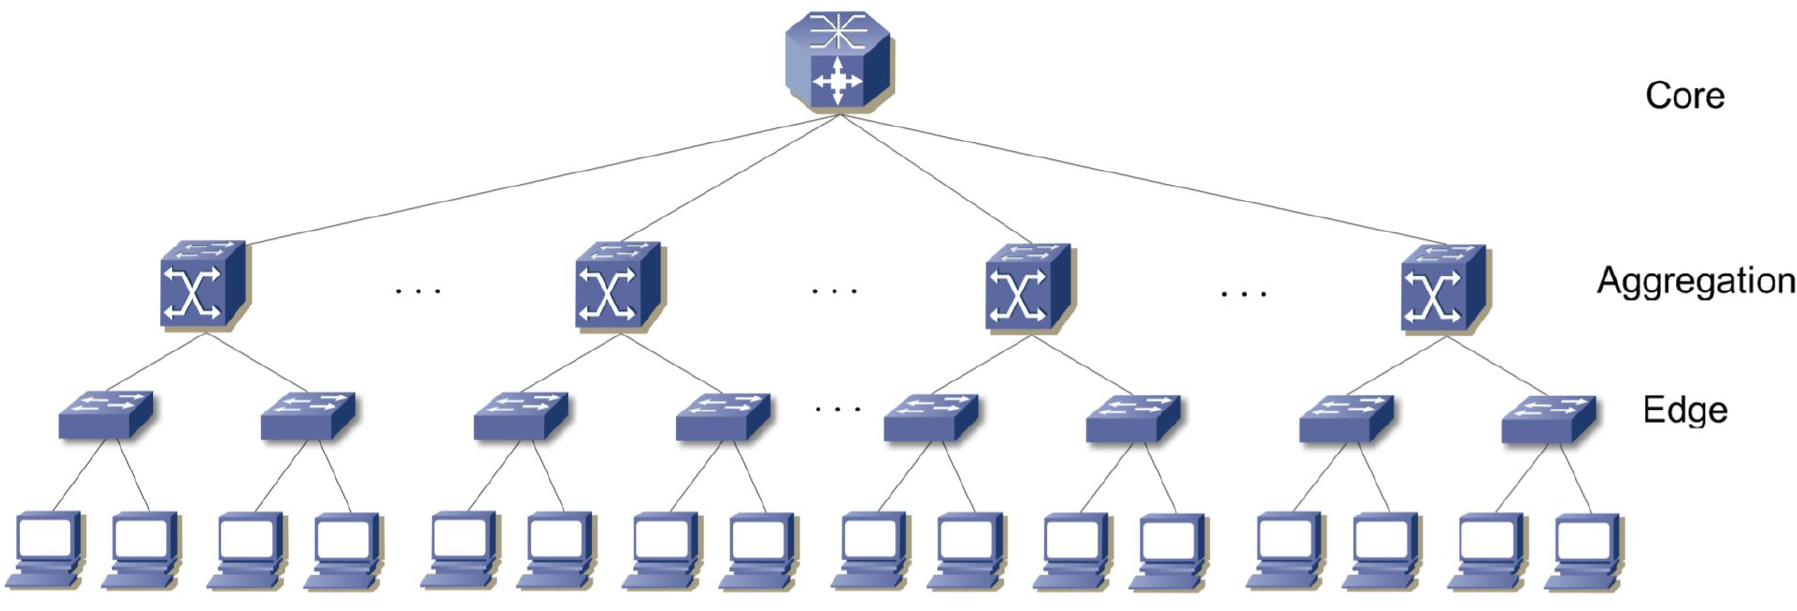
\includegraphics[scale=0.5]{../../immagini/dc_topology}
\end{figure}\\\\
ci sono diversi server che devono comunicare fra di loro e non con la rete esterna, ci sono diversi tiers
\begin{itemize}
    \item edge: prima rete attaccata ad un gruppo di server, sono degli switch di accesso anche detti top of racks, devono fare da accesso per il resto della rete di overlay
    \item aggregation switches, anche detti end of rack. 
    \\Raggruppano un certo numero di tor
    \item infine, i core switches.
    \\Devono essere più complessi e costosi, perché devono aggregare e processare tutto il traffico che viene forwardato sulla rete.
    \\Nell'aggregazione, occorre moltiplicare la bandwidth di ogni server che deve passare per lo switch, inoltre questi device hanno anche la connessione verso l'Internet
\end{itemize}
La limitazione di questa architettura è la over-subscription, ovvero la banda aggregata nel core può essere problematica per i cores, possono trovarsi a processare anche 1 Tbps di traffico ed inoltre non c'è tolleranza ai guasti fra i collegamenti dei core switches o sul core switch stesso.
\\Gli obiettivi chiave delle reti dei data center sono
\begin{itemize}
    \item scalabilità: i server possono aumentare e serve avere una rete che supporta questo aumento, senza incidere sull'architettura esistente
    \item ridondanza, principalmente per la tolleranza ai guasti.
    \\Non ci può essere un single point of failure
    \item latenza, dipende dal numero di hops che c'è nel data center
    \item capacità della rete, in base all'applicazione 
    \item tenants isolation, che riguarda più che altro le applicazioni cloud.
    \\La sicurezza e l'isolamento deve essere supportata anche da un punto di vista della rete.
\end{itemize}

\subsection{clos topology - 2 tier}
Oggi la topologia usata è la rete con topologia clos, più comune in due tier (nota anche come leaf-spine).
\\Si può avere anche un caso 3-tier, anche detta fat-tree.
\\Un caso di two-tier è il seguente:\\
\begin{figure}[h!]
    \centering
    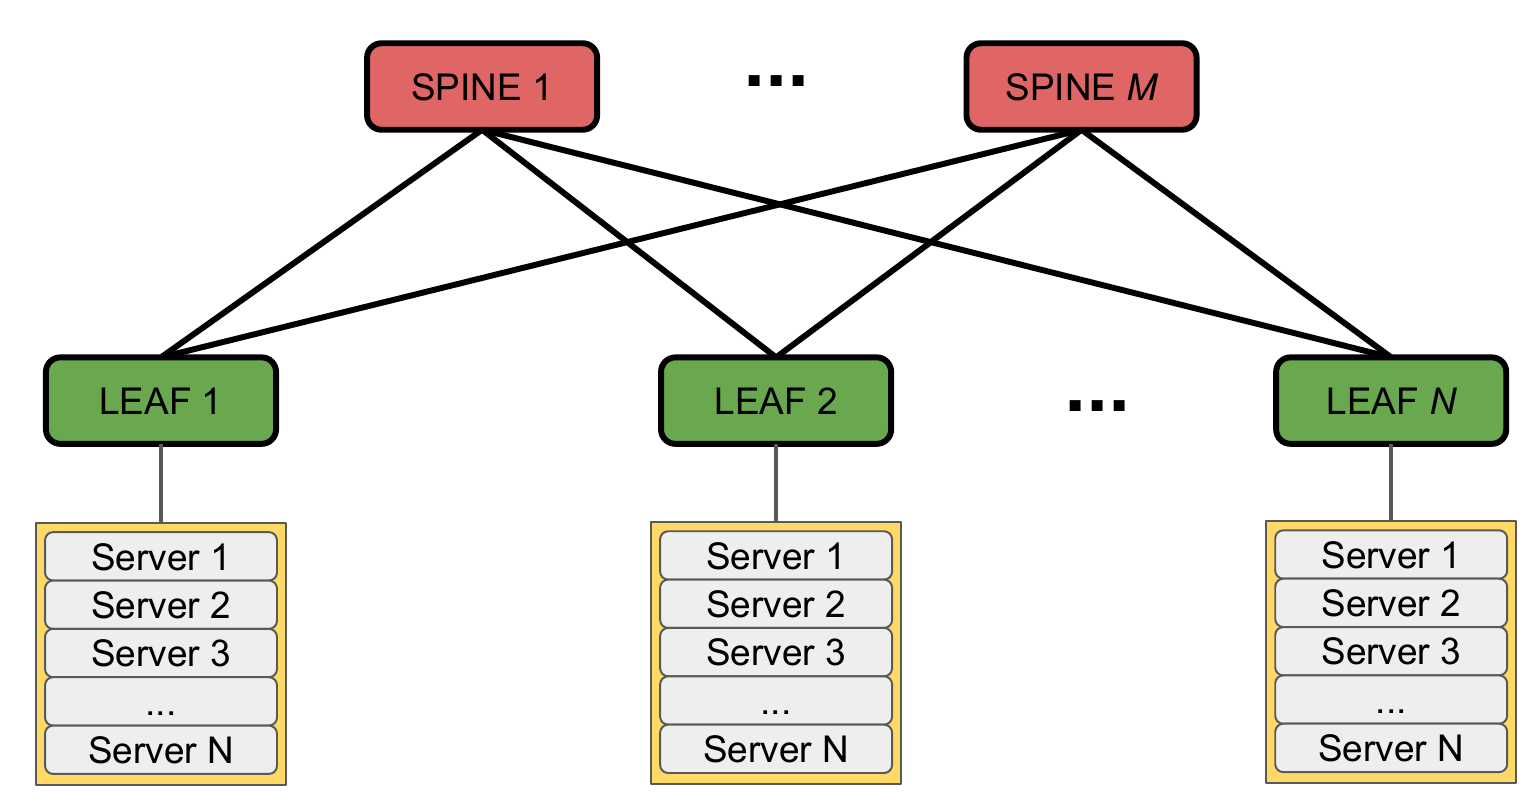
\includegraphics[scale=0.5]{../../immagini/2tear_ls}
\end{figure}\\\\
è utile in quanto se serve avere più banda, basta aggiungere una spine in più e collegarla alle foglie, se servono più server basta aggiungere una foglia e connetterla alla spina.
\\Per la fault tollerance
\begin{itemize}
    \item se una spina fallisce, siccome la connessione delle foglie è verso tutte le spine c'è comunque raggiungibilità (un fault può essere anche un update software che può durare per molto, ad esempio 5 min).
    \\Ci sono anche protocolli che riconoscono i fallimenti e redirigono il traffico verso le altre spine
    \item se fallisce una foglia, avendo una sola foglia non si può più raggiungere il mondo esterno.
\end{itemize}

Ci sono quindi protocolli per la fault tollerance, per le foglie:
\begin{itemize}
    \item lag: tecnica di multiplexing inversa.
    \\Qui, configuriamo più link per avere virtualmente un link, il protocollo gestisce il fallimento fra i link che vengono configurati.
    \\La ridondanza viene fatta per la fault tollerance;
    \item mlag: ridondanza a livello di switch, compriamo due foglie e configuriamo un numero di link verso le due foglie (i due link sono p2p link) e viene fatto per avere ridondanza anche a livello di switch.
\end{itemize}
Se il processamento è sempre lo stesso, la latenza dipende dal numero di hops che si hanno nella rete.
\\La latenza deve essere fissata, almeno per quanto riguarda il numero di hop, quindi non solo latenza bassa ma anche fissa in quanto ci aspettiamo un certo valore.
\\Il numero di hops fra un end-host ed un altro è chiamato diametro di rete.
\\Per la larghezza di banda, c'è il bi-section bandwidth: questa è la banda minima quando metà dei nodi della rete sta mandando simultaneamente alla massima capacità del link dati verso gli altri nodi.
\\L'oversubscription ratio è il ratio fra il peggiore danwidth aggregato raggiungibile fra due end-host diviso per il bisection bandwidth.
\\Sia N il numero di end-nodes e B bit/s la capacità dei link fra end-nodes, allora la condizione ideale è
\begin{equation}
    Bisection bandwidth = \frac{N}{2} \cdot B
\end{equation}

Normalmente, le reti con una topologia tier-2 prevede due foglie che mantengono solo la connessione verso Internet

\subsection{clos topology - 3 tier}
La fat-tree è sviluppata su 3 tier, possiamo vederla come se venga esploso una foglia in un gruppo di 4 foglie, chiamate pots.
\\Abbiamo la seguente struttura\\
\begin{figure}[h!]
    \centering
    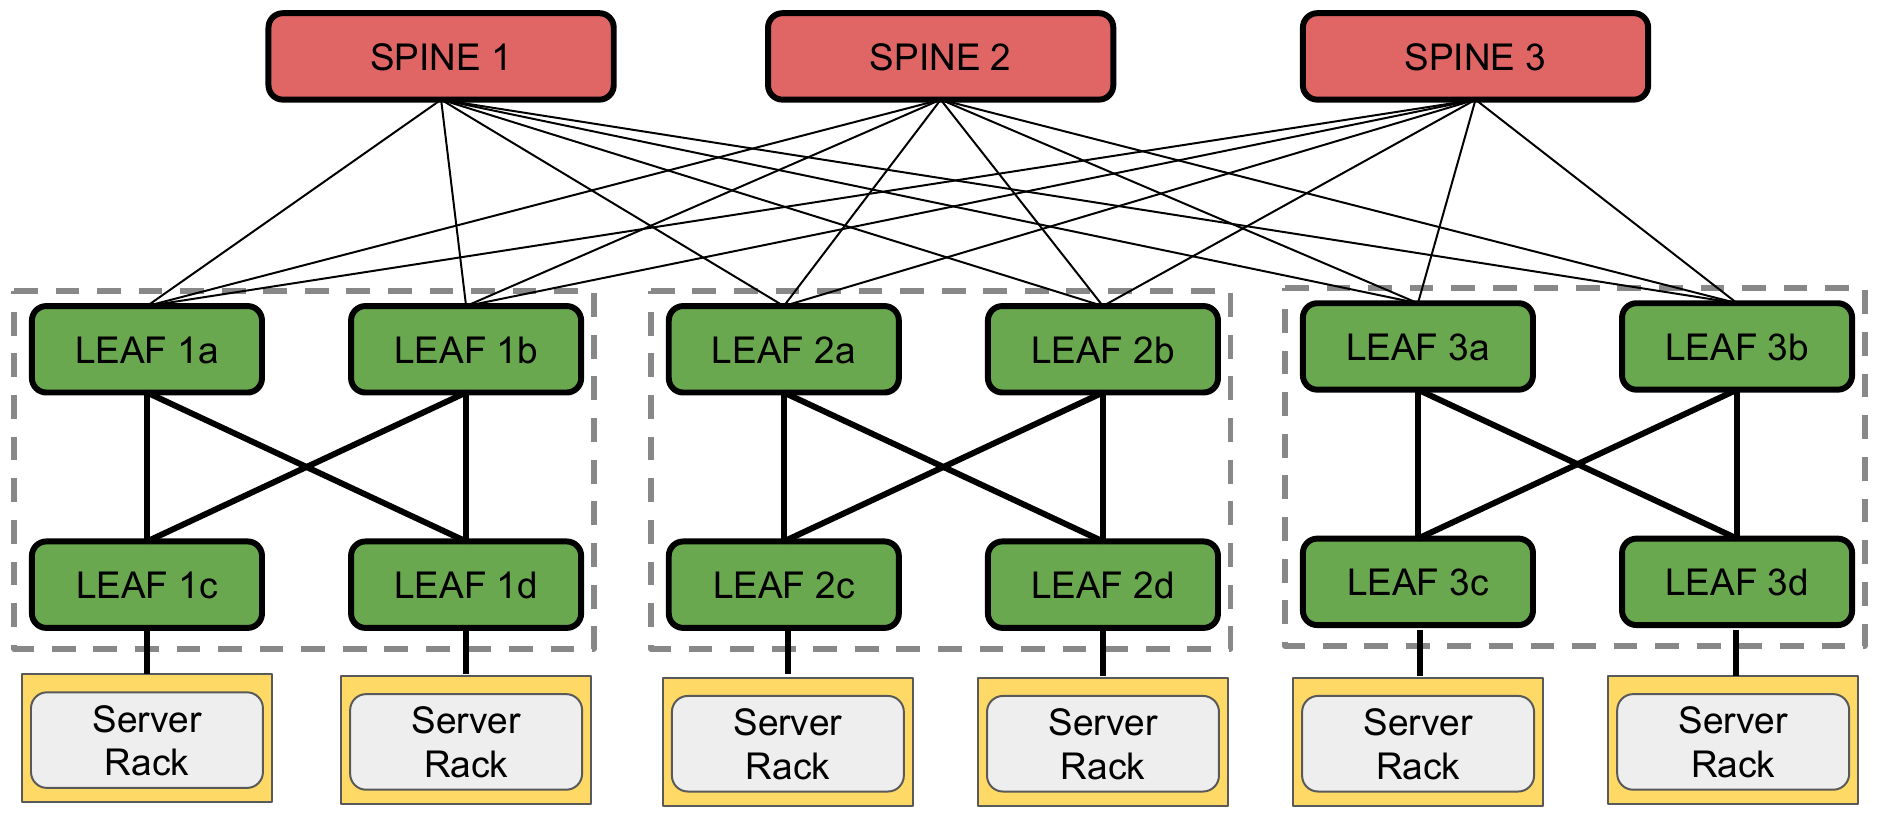
\includegraphics[scale=0.5]{../../immagini/fat_tree}
\end{figure}

\section{VXLAN}
Nella topologia a 2-tier vogliamo, siccome ci sono link ridondati, load balancing.
\\Se abbiamo m spine, ci sono m spine differenti per ogni end-node, quindi se abbiamo 5 foglie ci sono 5 path differenti fra cui scegliere.
\\Non possiamo avere load balancing nelle reti L2 per via del protocollo spanning tree, quindi non possiamo avere una rete L2 fra foglie e spine.
\\Un'altra limitazione importante è che per la virtualizzazione le vlans sono molto limitate, non solo per via di ipv4 vs ipv6 ma proprio perché ci sono massimo 4000 identificatori di rete fra cui scegliere.
\\Quindi, per la virtualizzazione delle reti si sceglie il forwarding L3, creiamo dei tunnel L3 in cui possiamo redirigere il traffico delle vm.
\\La multi-tenancy è l'abilità del cloud provider di isolare i diversi client anche se condividono la stessa infrastruttura, un altro requisito che si ha nella multi-tenancy è che si possano riusare i MAC address, quindi i frame L2 devono essere incapsulati in un tunnel L3.
\\Il protocollo di incapsulamento più usato è VXLAN (virtual extensible local area network), si può vedere come una estensione di vlan, in quanto estende il numero di identificatori fino a 24 bit.
\\VXLAN può funzionare anche in reti non-IP, in quanto è indipendente dalla rete L3 sottostante (mentre con VPN-MPLS serve essere basati su IP).
\\Opera a livello 3, avremo un incapsulamento IP/UDP ed ogni router sa come fare load balancing di un pacchetto IP/UDP.
\\Un'altra feature è che solo i nodi edge possono supportare l'incapsulamento, il tunnel è solo fra loro.
\\Questo è un esempio di pacchetto:\\
outer l2 header $||$ outer ip header $||$outer UDP header $||$VXLAN header $||$ original L2 frame\\
in una leaf spine, abbiamo inizializzazione e terminazione del tunnel chiamate vteps, a cui spetta il compito di incapsulare ed istanziare i pacchetti.
\\L'indirizzo sorgente che abbiamo nel IP header più esterno è quello del nodo foglia che inizializza il tunnel, la destinazione è quella del vtep di dove è il server che viene contattato.
\\La porta sorgente può essere scelta dal vtep, mentre la porta destinazione è fissata, abbiamo poi gli header vxlan che hanno alcuni header fra cui il \texttt{vni} ovvero l'identificatore della vxlan.
\\Stiamo incapsulando un frame l2 in una rete di overlay l3, ma anche vxlan può essere usata per vpn di livello 3, come abbiamo visto per mpls.
\\L'l2vni è associato ad un dominio di broadcast, quindi virtualmente connesso ad uno switch e che ha una certa vlan.
\\Possiamo avere un tenant con diverse sotto-reti, lo use case può essere di comunicare fra le diverse subnet, quindi non si usa lo stesso dominio broadcast ma si crea una vpn identificata come l3vni: abbiamo il frame l2 nel pacchetto vxlan, ma il forwarding è a livello 3, si manda un pacchetto da un dominio broadcast verso un altro. (possiamo vedere l3vni come il route distinguisher).

\subsection{Load balancing: ecmp}
La soluzione più usata è ecmp, è una tecnica semplice per cui normalmente si prendono le 5-tuple
\begin{itemize}
    \item ip src/dest
    \item port src/dest
    \item protocollo
\end{itemize}
si fa l'hash delle tuple, si taglia il digest in base al numero totale delle interfacce e basandosi sul valore che si ha nei bucket hash si sceglie un next hop.
\\Si aggiunge la complessità dell'hash perché se si facesse un round robin con ciascun pacchetto, si manderebbe un burst in ciascun percorso ma se c'è congestione in uno dei link è possibile che il receiver riceva i pacchetti in ordine inverso, che può essere un problema perché ricevere traffico tcp in ordine inverso è un problema di performance importante nei data center.
\\Se c'è un flusso pesante, bandwidth angry, con ecmp viene sempre routato per lo stesso path e quindi non è facilmente redirigibile in un altro path.
\\Per essere compatibile con tutti in nodi nella rete, non possiamo aspettarci che ogni nodo della rete verifichi nel vlan header: ecmp viene calcolato sull'header esterno per essere compatibile con tutti i nodi della rete.
\\Ma se la porta sorgente e destinazione sono sempre le stesse, applicando ecmp si sceglie sempre la stessa rotta, quindi si cambia la porta sorgente udp, non si può fare con round robin e quindi si sceglie in modo da avere delle informazioni riguardo il pacchetto all'interno dell'incapsulamento vxlan:
\begin{itemize}
    \item si fa un hash della 5-pla del frame l2 originale
    \item in base a questo, si seleziona la porta sorgente udp
\end{itemize}
in base al pacchetto sorgente, si riesce ad ottenere load balancing con ecmp.

\subsection{VXLAN VTEPS}
Per quello che abbiamo visto, i vteps sono switch foglie.
\\Gli switch foglie hanno sempre il supporto hardware per vxlan, se si vuole farlo anche negli end host occorre avere la capacità hardware nella nic, le operazioni di incapsulamento e de-capsulamento sono pesanti nel kernel e quindi ci sono tecnologie come open virutal switch per il processamento in vxlan.

\subsection{Utilizzi di vxlan}
Perché usare vxlan invece di mpls: la risposta più breve è che mpls non è stato progettato per questo scopo, in quanto l'obiettivo era quello di fare switching basandosi sul nuovo header mpls e non col longest prefix matching, ed inoltre mpls permette alle reti di diversi customers di essere routate nella rete Internet (??).
\\Non si può inoltre supportare frame l2 in una overlay di livello 3 con mpls, quindi avere due dominii broadcast nello stesso tenant.
\\(lab: tenants vms, il progetto è già scritto. è un favore che faccio al me del futuro che almeno c'avrà la topologia fatta. visto che st'homework 3 ti sta piegando in 3).


\section{Control plane di VXLAN: EVPN}
EVPN è il control plane per VXLAN, introdotto in quanto non era stato definito un control plane.
\\Le richieste ARP ed in generale tutto il mac flooding viene replicato nella rete di overlay, nel caso del laboratorio abbiamo un tunnel per tenant ma se fossero di più ogni volta che viene fatta una richiesta arp questa passa per tutti i tunnel l3 e quindi farebbe flooding anche a livello 3.
\\EVPN risolve i problemi delle vxlan statiche, usa il meccanismo di mpls-bgp, c'è una nuova famiglia di indirizzi bgp che vengono pubblicati e l'idea è che ogni terminazione esporterà alla rete bgp che ha un certo numero di tenants e quindi la scoperta è automatica e si possono importare gli annunci per le vpn che i vteps hanno dietro e questo riduce il traffico del flooding.
\\Le evpn più importanti sono
\begin{itemize}
    \item type 1: Ethernet auto-discovery route
    \item type 2: usata per advertising di indirizzi mac/ip.
    \\La rotta di tipo 2 è quindi una traduzione per installare entry arp dentro una vtep 
    \item type 3: messaggi per ethernet multicast, usati per scoprire le altre vtep
    \item type 4: si può fare advertising di una rete dietro la vtep, non solo gli host
    \item type 5: IP prefix route
\end{itemize}

\subsection{EVPN type 2}
Sono scambiati fra i vteps per fare advertising di indirizzi ip e mac.
\\Vogliamo sincronizzare, ricevendo ed inviando gli annunci fra vteps, le tabelle mac ed associazioni fra ip e mac (quindi le tabelle arp) della vni livello 2.
\\Ogni volta che la vtep impara un indirizzo, ovvero riceve un pacchetto verso un altro host, si manda l'update evpn.
\\In questo modo il traffico l2 non viene mandato in flooding, prima le richieste arp ed il mac learning erano in flooding quando non si conosceva l'indirizzo.
\\In questo caso, le rotte sono pre-installate nel bridge nella specifica vlan.
\\Nel pacchetto c'è il route distinguisher, ma non ha lo stesso valore che c'è nelle vpn mpls, che era usato per identificare una vpn, in questo caso dipende dall'implementazione.
\\Ci sono diversi scenari nel caso del livello 2
\begin{itemize}
    \item host arp advertisement, può avere due casi d'uso
    \begin{itemize}
        \item arp broadcast suppression, evitiamo di forwardare la richiesta arp.
        \\Quando una richiesta broadcast viene ricevuta dal vtep, il vtep connesso a quel dominio risponde come un proxy
        \item vm migration: quando avviene la migrazione fra vtep diversi, l'istanza evpn si rende conto del cambiamento del mac e triggera una richiesta arp per capire se è ancora nella sua rete e quando fallisce ritira le rotte in quanto ora vengono annunciate dal nuovo vtep che hosta la vm.
    \end{itemize}
\end{itemize}

\subsection{EVPN tipo 3}
Usate per mandare advertisement agli l2vni e gli IP dei vtep fra tutti i vtep per creare delle liste di replicazione.
\\Il tipo 3 è quindi usato per scoprire le terminazioni delle VXLAN di tutte le VPN l2 configurate nella rete di overlay BGP.
\\Quest'informazione è contenuta in un altro campo extended community di BGP detto PMSI.
\\Il formato è leggermente diverso
\begin{itemize}
\item flags
\item tunnel type
\item altro sulle slides
\end{itemize}

\subsection{EVPN tipo 5}
Sono simili alle tipo 2 per gli advertisement degli IP host di prefissi /32 o /128.
\\Nel caso di tipo 5, è possibile annunciare sottoreti con lunghezze di prefisso variabili.
\\Sono usate per mandare informazioni di raggiungibilità per l3nvi e non per domini di broadcast l2vni.
\\Quindi usate per il routing inter-sottorete fra le l2vni di uno stesso tenant.


\subsubsection{lab vxlan ebgp}
Il lab ha la stessa topologia di prima, quindi basta cambiare gli script.
\\Occorre rimuovere i tunnel statici e cambiarli con le implementazioni ebgp.
\\Per istanziare bgp, si può usare sia ibgp che ebgp, dipende dalle necessità.
\\Sta tutta sulle slides la configurazione.
\\Nota in più: per avere un indirizzo ip per la vtep, va configurato in cumulus per usarlo come default gateway per fargli routare il traffico. (ancora slides).
\\Vediamo cosa accade nel caso della migrazione di una vm: passiamo le vm da lubuntu1 a lubuntu3, per emulare la migrazione è cancellare i link e riconnetterli in maniera swappata (lubuntu1 si connette alla leaf3 e viceversa).
\\In automatico, evpn scambia le informazioni delle vm migrate e quindi che i mac sono cambiati e ci sono degli annunci scambiati nella rete.
\\\\Secondo laboratorio: stessa topologia, usando l3 vni. vogliamo emulare un singolo tentant, quindi uniamo i due precedenti in un unico:
\begin{itemize}
    \item vogliamo cambiare gli indirizzi
    \item dobbiamo creare una nuova rete per la vm b in quanto vogliamo avere il routing fra le due reti dello stesso tenant.
    \\Aggiungiamo quindi un'altra interfaccia vxlan, che implementa vni: manda i pacchetti a livello 3, quindi è simile ad una vpn mpls bgp.
\end{itemize}
Ci sono gli stessi indirizzi di default nei diversi vtep, serve per semplificare lo scenario ma è quello che si fa per implementare i vni.
\\Siamo in domini boradcast differenti, quindi dobbiamo fare la connessione a livello 3 e non più a livello 2.
\\Quindi creiamo con comando vrf una tabella di routing.
\\Abbiamo quindi creato un tunnel fra due diverse subnets, in questo senso è a livello 3 poiché è necessario che i pacchetti passino per un router affinché vengano instradati.

\end{document}
